% -----------------------------------------------------------------------------
% Apêndices
% -----------------------------------------------------------------------------

\begin{apendicesenv}
\partapendices

% -----------------------------------------------------------------------------
% Primeiro apêndice
% -----------------------------------------------------------------------------


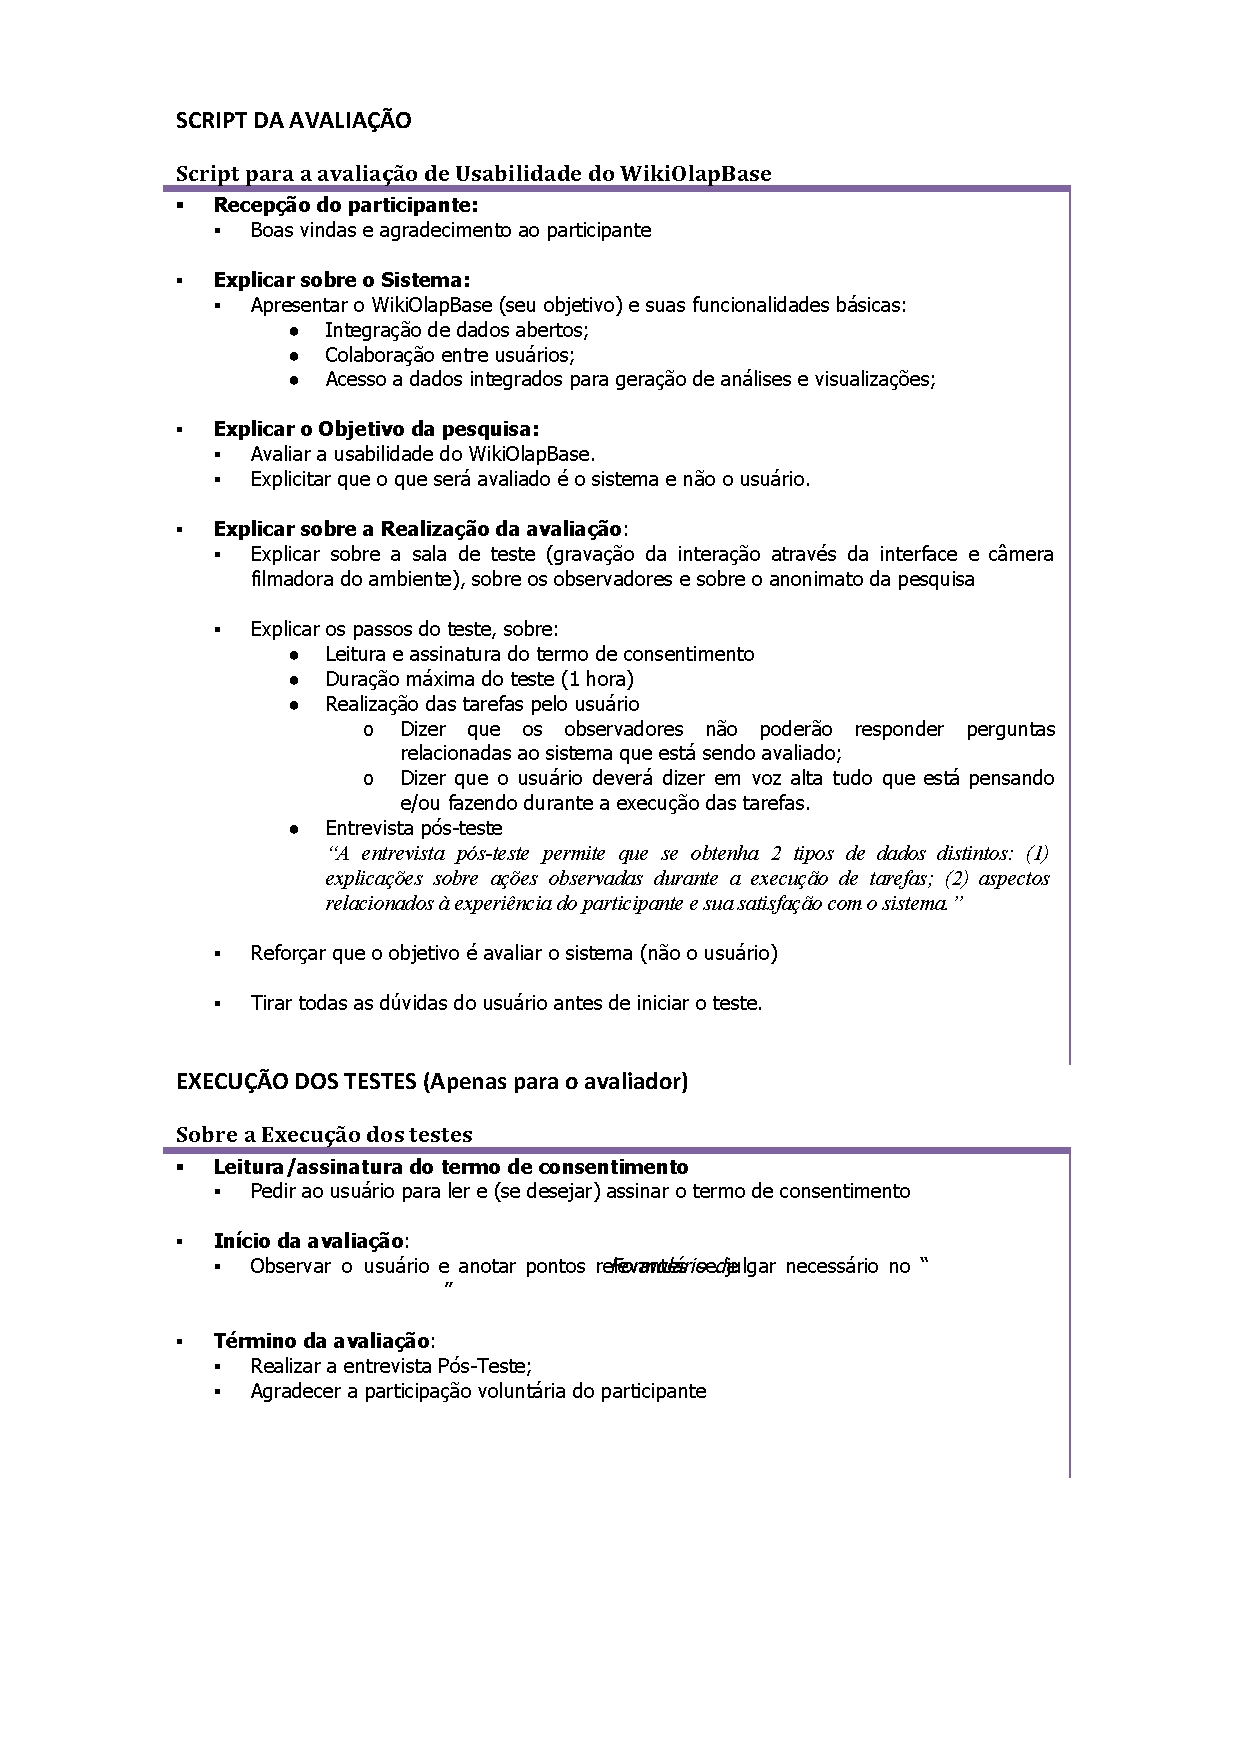
\includepdf[pages=1, scale=0.8,pagecommand=\chapter{Artefatos de Avaliação}\label{apendiceA}]{./04-figuras/avaliacao-artefatos}
\includepdf[pages=2-, scale=0.8, pagecommand={}]{./04-figuras/avaliacao-artefatos}

\chapter{Lista de Melhorias}
\label{apendiceB}

\begin{enumerate}  
    \item Criação de um sistema de cadastro e autenticação de usuários. 
    \item Adicionar suporte a outros formatos de arquivos. 
    \item Permitir o envio de arquivos compactados.
    \item Permitir o envio de múltiplos arquivos.
    \item Estender a função de busca para mostrar todos metadados.
    \item Incluir ícone na interface de editar nome das colunas para especificar a possibilidade de edição.
    \item Estender as funcionalidades da API para permitir outras operações e aplicação de filtros.
    \item Utilização de URIs para identifação das \textit{tags} das colunas. Utilizar, por exemplo, o schema.org.
\end{enumerate}

\end{apendicesenv}
